\section{Метод сопряженных градиентов}

\textbf{Алгоритм метода}:
$$ x^{k+1} = x^{k} + t_{k}d^{k}$$

$$ d^{0} = - \nabla f(x^{0})$$
$$ d^{k} = - \nabla f(x^{k}) + \beta_{k - 1}d^{k - 1}$$
$t_{k}$ --- шаг вычисляется из условия наибольшего убывания функции в точках последовательности: $t_{k} = argmin|f(x^{k+1})|$


Основной критерий окончания метода:$|| \nabla f(x^{k})|| < \varepsilon$.

Начальные параметры метода: $x^{0}, \varepsilon$.

Изменяемые параметры метода: отрезок для уточнения шага $[a, b]$.

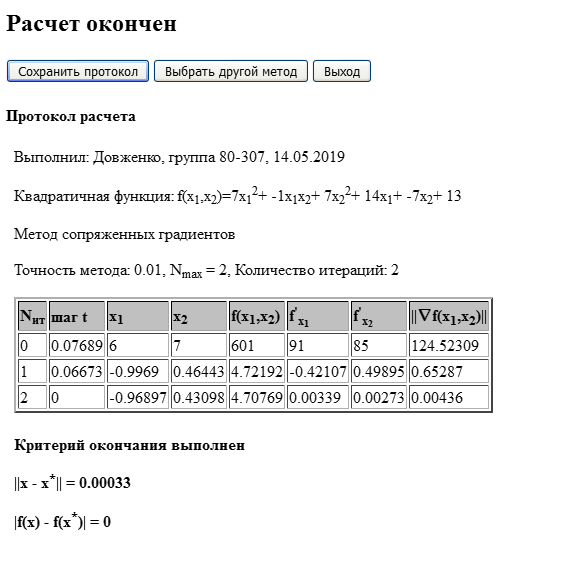
\includegraphics[width=0.8\linewidth]{om_hw_01/img/1.PNG}\\
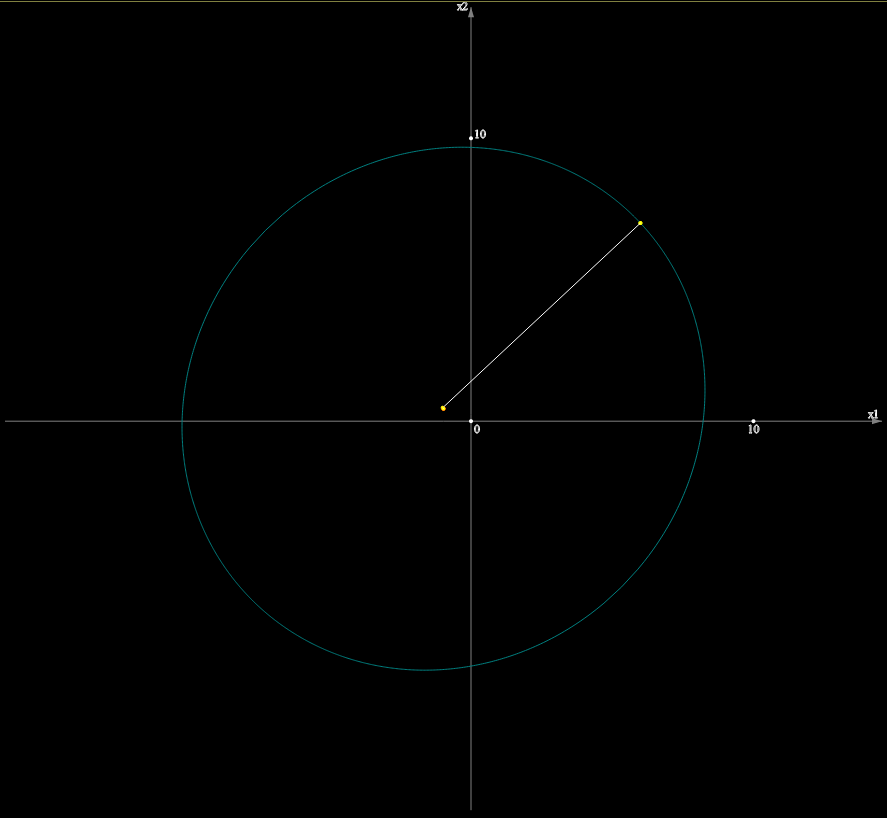
\includegraphics[width=0.6\linewidth]{om_hw_01/img/1_2.PNG}\\

\textbf{Последняя итерация}:

$x^{0}_{1} = N^{0} = 6$\\
$x^{0}_{2} = 7$\\
$x^{2} = x^{1} + t_{1} +d^{1}$\\
$
x^{1} = 
\begin{pmatrix}
  -0.9969\\
  0.46443
\end{pmatrix}
$\\
$t_{1} = 0.06673$\\
$d^{1} = -\nablaf(x^{1}) + B_{0}d^{0}$\\
$d^{0} = -\nablaf(x^{0})$\\
$B_{0} = \dfrac{||\nabla f(x^{1})||^{2}}{||\nabla f(x^{0})||^{2}} = \dfrac{(0.65287)^{2}}{(124.52309)^{2}} = 0.0000274$\\
$
\nabla f = 
\begin{pmatrix}
  14x_{1} - x_{2} + 14\\
  14x_{2} - x_{1} - 7
\end{pmatrix}
$\\
$
\nabla f(x^{0}) = 
\begin{pmatrix}
  91\\
  85
\end{pmatrix}
$\\
$
\nabla f(x^{1}) = 
\begin{pmatrix}
  -0.421\\
  0.4985
\end{pmatrix}
$\\
Тогда\\
$
d^{1} = 
\begin{pmatrix}
  0.421\\
  -0.4985
\end{pmatrix}
+
\begin{pmatrix}
  -0.00249\\
  -0.00232
\end{pmatrix}
=
\begin{pmatrix}
  0.41851\\
  -0.50082
\end{pmatrix}
$\\

$
x^{2} = 
\begin{pmatrix}
  -0.9969\\
  0.46443
\end{pmatrix}
+ 0.06673
\begin{pmatrix}
  0.41851\\
  -0.50082
\end{pmatrix}
=
\begin{pmatrix}
  -0.96897\\
  0.43101
\end{pmatrix}
$

\pagebreak